\documentclass[journal,12pt,twocolumn]{IEEEtran}
\usepackage{setspace}
\usepackage{gensymb}
\usepackage{caption}
%\usepackage{multirow}
%\usepackage{multicolumn}
%\usepackage{subcaption}
%\doublespacing
\singlespacing
\usepackage{csvsimple}
\usepackage{amsmath}
\usepackage{multicol}
%\usepackage{enumerate}
\usepackage{amssymb}
%\usepackage{graphicx}
\usepackage{newfloat}
%\usepackage{syntax}
\usepackage{listings}
\usepackage{color}
\usepackage{tikz}
\usepackage{graphicx}
\usetikzlibrary{shapes,arrows}

%\usepackage{graphicx}
%\usepackage{amssymb}
%\usepackage{relsize}
%\usepackage[cmex10]{amsmath}
%\usepackage{mathtools}
%\usepackage{amsthm}
%\interdisplaylinepenalty=2500
%\savesymbol{iint}
%\usepackage{txfonts}
%\restoresymbol{TXF}{iint}
%\usepackage{wasysym}
\usepackage{amsthm}
\usepackage{mathrsfs}
\usepackage{txfonts}
\usepackage{stfloats}
\usepackage{cite}
\usepackage{cases}
\usepackage{mathtools}
\usepackage{caption}
\usepackage{enumerate}	
\usepackage{enumitem}
\usepackage{amsmath}
%\usepackage{xtab}
\usepackage{longtable}
\usepackage{multirow}
%\usepackage{algorithm}
%\usepackage{algpseudocode}
\usepackage{enumitem}
\usepackage{mathtools}
\usepackage{hyperref}
%\usepackage[framemethod=tikz]{mdframed}
\usepackage{listings}
    %\usepackage[latin1]{inputenc}                                 %%
    \usepackage{color}                                            %%
    \usepackage{array}                                            %%
    \usepackage{longtable}                                        %%
    \usepackage{calc}                                             %%
    \usepackage{multirow}                                         %%
    \usepackage{hhline}                                           %%
    \usepackage{ifthen}                                           %%
  %optionally (for landscape tables embedded in another document): %%
    \usepackage{lscape}     


\usepackage{url}
\def\UrlBreaks{\do\/\do-}


%\usepackage{stmaryrd}


%\usepackage{wasysym}
%\newcounter{MYtempeqncnt}
\DeclareMathOperator*{\Res}{Res}
%\renewcommand{\baselinestretch}{2}
\renewcommand\thesection{\arabic{section}}
\renewcommand\thesubsection{\thesection.\arabic{subsection}}
\renewcommand\thesubsubsection{\thesubsection.\arabic{subsubsection}}

\renewcommand\thesectiondis{\arabic{section}}
\renewcommand\thesubsectiondis{\thesectiondis.\arabic{subsection}}
\renewcommand\thesubsubsectiondis{\thesubsectiondis.\arabic{subsubsection}}

% correct bad hyphenation here
\hyphenation{op-tical net-works semi-conduc-tor}

%\lstset{
%language=C,
%frame=single, 
%breaklines=true
%}

%\lstset{
	%%basicstyle=\small\ttfamily\bfseries,
	%%numberstyle=\small\ttfamily,
	%language=Octave,
	%backgroundcolor=\color{white},
	%%frame=single,
	%%keywordstyle=\bfseries,
	%%breaklines=true,
	%%showstringspaces=false,
	%%xleftmargin=-10mm,
	%%aboveskip=-1mm,
	%%belowskip=0mm
%}

%\surroundwithmdframed[width=\columnwidth]{lstlisting}
\def\inputGnumericTable{}                                 %%
\lstset{
%language=C,
frame=single, 
breaklines=true,
columns=fullflexible
}

\begin{document}
%
\tikzstyle{block} = [rectangle, draw,
    text width=3em, text centered, minimum height=3em]
\tikzstyle{sum} = [draw, circle, node distance=3cm]
\tikzstyle{input} = [coordinate]
\tikzstyle{output} = [coordinate]
\tikzstyle{pinstyle} = [pin edge={to-,thin,black}]

\theoremstyle{definition}
\newtheorem{theorem}{Theorem}[section]
\newtheorem{problem}{Problem}
\newtheorem{proposition}{Proposition}[section]
\newtheorem{lemma}{Lemma}[section]
\newtheorem{corollary}[theorem]{Corollary}
\newtheorem{example}{Example}[section]
\newtheorem{definition}{Definition}[section]
%\newtheorem{algorithm}{Algorithm}[section]
%\newtheorem{cor}{Corollary}
\newcommand{\BEQA}{\begin{eqnarray}}
\newcommand{\EEQA}{\end{eqnarray}}
\newcommand{\define}{\stackrel{\triangle}{=}}

\bibliographystyle{IEEEtran}
%\bibliographystyle{ieeetr}

\providecommand{\nCr}[2]{\,^{#1}C_{#2}} % nCr
\providecommand{\nPr}[2]{\,^{#1}P_{#2}} % nPr
\providecommand{\mbf}{\mathbf}
\providecommand{\pr}[1]{\ensuremath{\Pr\left(#1\right)}}
\providecommand{\qfunc}[1]{\ensuremath{Q\left(#1\right)}}
\providecommand{\sbrak}[1]{\ensuremath{{}\left[#1\right]}}
\providecommand{\lsbrak}[1]{\ensuremath{{}\left[#1\right.}}
\providecommand{\rsbrak}[1]{\ensuremath{{}\left.#1\right]}}
\providecommand{\brak}[1]{\ensuremath{\left(#1\right)}}
\providecommand{\lbrak}[1]{\ensuremath{\left(#1\right.}}
\providecommand{\rbrak}[1]{\ensuremath{\left.#1\right)}}
\providecommand{\cbrak}[1]{\ensuremath{\left\{#1\right\}}}
\providecommand{\lcbrak}[1]{\ensuremath{\left\{#1\right.}}
\providecommand{\rcbrak}[1]{\ensuremath{\left.#1\right\}}}
\theoremstyle{remark}
\newtheorem{rem}{Remark}
\newcommand{\sgn}{\mathop{\mathrm{sgn}}}
\providecommand{\abs}[1]{\left\vert#1\right\vert}
\providecommand{\res}[1]{\Res\displaylimits_{#1}} 
\providecommand{\norm}[1]{\left\Vert#1\right\Vert}
\providecommand{\mtx}[1]{\mathbf{#1}}
\providecommand{\mean}[1]{E\left[ #1 \right]}
\providecommand{\fourier}{\overset{\mathcal{F}}{ \rightleftharpoons}}
%\providecommand{\hilbert}{\overset{\mathcal{H}}{ \rightleftharpoons}}
\providecommand{\system}{\overset{\mathcal{H}}{ \longleftrightarrow}}
	%\newcommand{\solution}[2]{\textbf{Solution:}{#1}}
\newcommand{\solution}{\noindent \textbf{Solution: }}
\newcommand{\myvec}[1]{\ensuremath{\begin{pmatrix}#1\end{pmatrix}}}
\providecommand{\dec}[2]{\ensuremath{\overset{#1}{\underset{#2}{\gtrless}}}}
\DeclarePairedDelimiter{\ceil}{\lceil}{\rceil}
%\numberwithin{equation}{section}
%\numberwithin{problem}{subsection}
%\numberwithin{definition}{subsection}
\makeatletter
\@addtoreset{figure}{section}
\makeatother

\let\StandardTheFigure\thefigure
%\renewcommand{\thefigure}{\theproblem.\arabic{figure}}
\renewcommand{\thefigure}{\thesection}


%\numberwithin{figure}{subsection}

%\numberwithin{equation}{subsection}
%\numberwithin{equation}{section}
%\numberwithin{equation}{problem}
%\numberwithin{problem}{subsection}
\numberwithin{problem}{section}
%%\numberwithin{definition}{subsection}
%\makeatletter
%\@addtoreset{figure}{problem}
%\makeatother
\makeatletter
\@addtoreset{table}{section}
\makeatother

\let\StandardTheFigure\thefigure
\let\StandardTheTable\thetable
\let\vec\mathbf
\numberwithin{equation}{section}

\vspace{3cm}


\title{%Convex Optimization in Python
	Random Numbers
}
%\title{
%	\logo{Matrix Analysis through Octave}{\begin{center}\includegraphics[scale=.24]{tlc}\end{center}}{}{HAMDSP}
%}

% paper title
% can use linebreaks \\ within to get better formatting as desired
%\title{Matrix Analysis through Octave}
%
%
% author names and IEEE memberships
% note positions of commas and nonbreaking spaces ( ~ ) LaTeX will not break
% a structure at a ~ so this keeps an author's name from being broken across
% two lines.
% use \thanks{} to gain access to the first footnote area
% a separate \thanks must be used for each paragraph as LaTeX2e's \thanks
% was not built to handle multiple paragraphs
%

\author{JARPULA BHANU PRASAD - AI21BTECH11015}
\maketitle

\tableofcontents

\bigskip

\renewcommand{\thefigure}{\theenumi}
\renewcommand{\thetable}{\theenumi}

\begin{abstract}
This manual provides a simple introduction to the generation of random numbers
\end{abstract}
%%
\section{Uniform Random Numbers}
Let $U$ be a uniform random variable between 0 and 1.
\begin{enumerate}[label=\thesection.\arabic*
,ref=\thesection.\theenumi]
\item Generate $10^6$ samples of $U$ using a C program and save into a file called uni.dat .\\
\solution
Download the following files and execute the C program
\begin{lstlisting}
$ wget https://github.com/jarpula-Bhanu/Random-numbers/blob/main/codes/exrand.c
$ wget https://github.com/jarpula-Bhanu/Random-numbers/blob/main/codes/coeffs.h
\end{lstlisting}
Compile and execute the above C program using command
\begin{lstlisting}
$ gcc exrand.c -lm -o exrand.out
$ ./exrand.out
\end{lstlisting}

%
\item
Load the uni.dat file into python and plot the empirical CDF of $U$ using the samples in uni.dat. The CDF is defined as
\begin{align}
F_{U}(x) = \pr{U \leq x}
\end{align}

\solution  The following code plots Fig. \ref{fig:uni_cdf}
\begin{lstlisting}
$ wget https://github.com/jarpula-Bhanu/Random-numbers/blob/main/codes/cdf_plot.py
\end{lstlisting}
The above code is executed using command
\begin{lstlisting}
$ python3 cdf_plot.py
\end{lstlisting}

\begin{figure}[h]
\centering
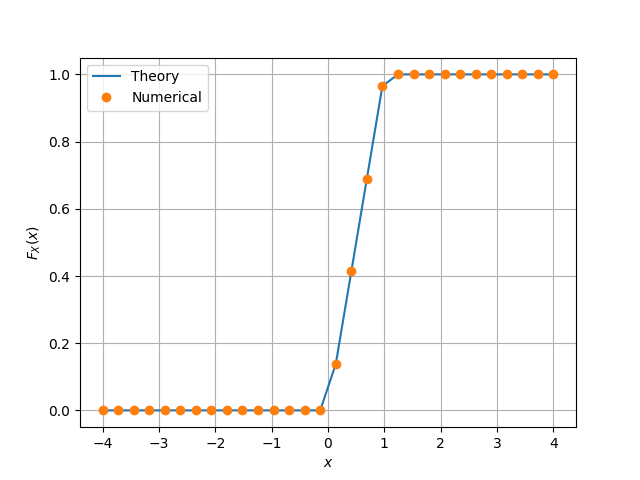
\includegraphics[width=\columnwidth]{uni_cdf.png}
\caption{The CDF of $U$}
\label{fig:uni_cdf}
\end{figure}

%
\item
Find a theoretical expression for $F_{U}(x)$.

\solution Since $U$ is a uniformly distributed in [0,1]  \\
We have three cases:
\begin{itemize}
\item $x < 0$: $P_X(x) = 0$, and hence $F_U(x) = 0$.
\item $0 \leq x < 1$: Here,
\begin{align}
    F_U(x) = \int_{0}^{x}du = x
\end{align}
\item $x \geq 1$: Put $x = 1$ in above eqn we get $F_U(x) = 1$.
\end{itemize}
Therefore,
\begin{align}
    F_U(x) = 
    \begin{cases}
        0 & x < 0 \\
        x & 0 \leq x < 1 \\
        1 & x \geq 1
    \end{cases}
\end{align}
This can be verified from Fig. \ref{fig:uni_cdf} 

\item
The mean of $U$ is defined as
%
\begin{equation}
E\sbrak{U} = \frac{1}{N}\sum_{i=1}^{N}U_i
	\label{eq:mean-form}
\end{equation}
%
and its variance as
%
\begin{equation}
\text{var}\sbrak{U} = E\sbrak{U- E\sbrak{U}}^2 
	\label{eq:var-form}
\end{equation}

Write a C program to  find the mean and variance of $U$.

\solution Download the following files and execute the C program
\begin{lstlisting}
$ wget https://github.com/jarpula-Bhanu/Random-numbers/blob/main/codes/exrand.c
$ wget https://github.com/jarpula-Bhanu/Random-numbers/blob/main/codes/coeffs.h
\end{lstlisting}
Compile and execute the above C program using command
\begin{lstlisting}
$ gcc exrand.c -lm -o exrand.out
$ ./exrand.out
\end{lstlisting}

The mean of $U$ is 0.500007\\
The varience of $U$ is 0.083301 \\

\item Verify your result theoretically given that
\end{enumerate}
%
\begin{equation}
E\sbrak{U^k} = \int_{-\infty}^{\infty}x^kdF_{U}(x)dx
\end{equation}
\solution Verifying result theoritically\\
Given that
\begin{align}
    E[U^k] &= \int_{-\infty}^{\infty} x^k dF_U(x)
\end{align}
Mean is given by
\begin{align}
    E[U] &= \int_{-\infty}^{\infty} x dF_U(x) \\
    &= \int_{-\infty}^{\infty} x dx \\
    &= \bigg[\frac{x^2}{2}\bigg]_0^1 \\
    &= \frac{1}{2}
\end{align}
Varaience is given by
\begin{align}
    E[U-E[U]]^2 &= E[U^2] - E[U]^2 \\
    E[U]^2 &= \int_{-\infty}^{\infty} x^2 dF_U(x)\\
    &= \int_{-\infty}^{\infty} x^2 dx \\
    &= \bigg[\frac{x^3}{3}\bigg]_0^1 \\
    &= \frac{1}{3} \\
    E[U-E[U]]^2 &= \frac{1}{3} - (\frac{1}{2})^2 \\
    &= \frac{1}{3} - \frac{1}{4} \\
    &= \frac{1}{12}
\end{align}
\section{Central Limit Theorem}
%
\begin{enumerate}[label=\thesection.\arabic*
,ref=\thesection.\theenumi]

%
\item
Generate $10^6$ samples of the random variable
%
\begin{equation}
X = \sum_{i=1}^{12}U_i -6
\end{equation}
%
using a C program, where $U_i, i = 1,2,\dots, 12$ are  a set of independent uniform random variables between 0 and 1
and save in a file called gau.dat

\solution
Download the following files and execute the C program
\begin{lstlisting}
$ wget https://github.com/jarpula-Bhanu/Random-numbers/blob/main/codes/exrand.c
$ wget https://github.com/jarpula-Bhanu/Random-numbers/blob/main/codes/coeffs.h
\end{lstlisting}
Compile and execute the above C program using command
\begin{lstlisting}
$ gcc exrand.c -lm -o exrand.out
$ ./exrand.out
\end{lstlisting}
%
\item
Load gau.dat in python and plot the empirical CDF of $X$ using the samples in gau.dat. What properties does a CDF have?

\solution The CDF of $X$ is plotted in Fig. \ref{fig:gauss_cdf}
\begin{figure}[h]
    \centering
    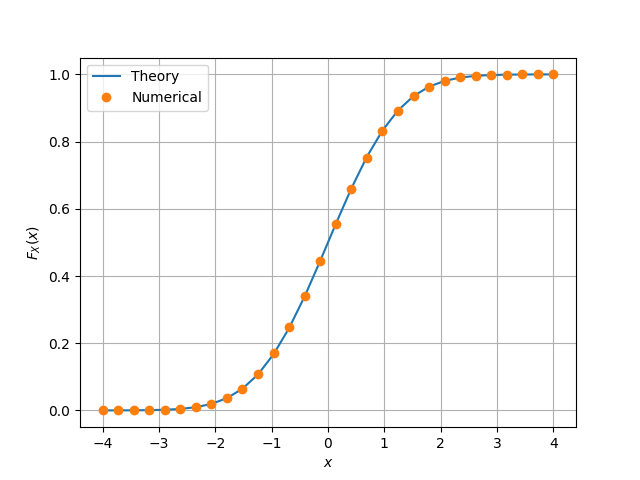
\includegraphics[width=\columnwidth]{gauss_cdf.png}
    \caption{The CDF of $X$}
    \label{fig:gauss_cdf}
\end{figure}
\textbf{properties of cdf}
\begin{itemize}
    \item $F_X(x)$ is a nondecreasing function of x for -$\infty < x < \infty$. 
    \item The CDF, $F_X(x)$ ranges from 0 to 1. This makes sense since $F_X(x)$ is a probability.
    \item If the maximum value of $X$ is b, then $F_X(b)$ = 1 \\
\end{itemize} 

\item
Load gau.dat in python and plot the empirical PDF of $X$ using the samples in gau.dat. The PDF of $X$ is defined as
\begin{align}
p_{X}(x) = \frac{d}{dx}F_{X}(x)
\end{align}
What properties does the PDF have?

\solution The PDF of $X$ is plotted in Fig. \ref{fig:gauss_pdf}
using the code below \\
Python code - \href{https://github.com/jarpula-Bhanu/Random-numbers/blob/main/codes/pdf_plot.py}{pdf\_plot.py}\\
The above code is executed using command
\begin{itemize}
    \item python3 pdf\_plot.py \\
\end{itemize}
\begin{figure}[h]
    \centering
    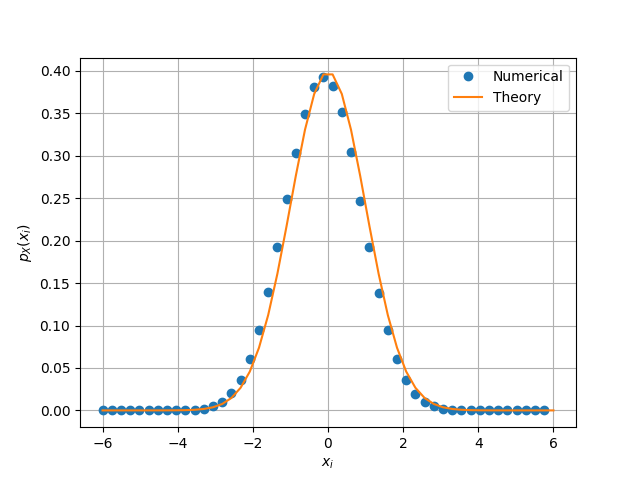
\includegraphics[width=\columnwidth]{gauss_pdf.png}
    \caption{The PDF of $X$}
    \label{fig:gauss_pdf}
\end{figure}

\textbf{properties of pdf}
\begin{itemize}
    \item PDF is symmetric about $X$ = 0 
    \item Graph is bell shaped
    \item Mean of graph is situated at the apex point of the bell.\\
\end{itemize}

\item Find the mean and variance of $X$ by writing a C program.

\solution
Download and run the following C code.

\noindent The C program can be downloaded using
\begin{lstlisting}
$ wget https://github.com/jarpula-Bhanu/Random-numbers/blob/main/codes/mean-var2-4.c
$ wget https://github.com/jarpula-Bhanu/Random-numbers/blob/main/codes/coeffs.h
\end{lstlisting}
Compile and execute the above C program using command
\begin{lstlisting}
$ gcc mean-var2-4.c -lm -o mean-var2-4.out
$ ./mean-var2-4.out
\end{lstlisting}

The mean of $X$ is 0.000326\\
The varience of $X$ is 1.000907\\

\item Given that 
\begin{align}
p_{X}(x) = \frac{1}{\sqrt{2\pi}}\exp\brak{-\frac{x^2}{2}}, -\infty < x < \infty,
\end{align}
repeat the above exercise theoretically.

\solution Verifying theoritically
    \begin{align}
        F_X(x) &= \int_{-\infty}^{x}\frac{1}{\sqrt{2\pi}}e^{-\frac{x^2}{2}}dx \\
        E[X]&= \frac{1}{\sqrt{2\pi}} \int_{-\infty}^{\infty}xe^{-\frac{x^2}{2}}dx 
    \end{align}
    Taking $\frac{x^2}{2} = t \rightarrow xdx = dt$
    \begin{align}
        E[X]&= \frac{1}{\sqrt{2\pi}} \int_{-\infty}^{\infty}e^{-t} dt = 0 \\
        E[X^2]&= \frac{1}{\sqrt{2\pi}} \int_{-\infty}^{\infty}x^2e^{-\frac{x^2}{2}}dx \\
        &= \frac{1}{\sqrt{2\pi}} \int_{-\infty}^{\infty}x(xe^{-\frac{x^2}{2}})dx \\
        &= \frac{1}{\sqrt{2\pi}} \bigg[-xe^{\frac{x^2}{2}}+\int_{-\infty}^{\infty}e^{-\frac{x^2}{2}} dx \bigg]_{-\infty}^{\infty} \\
        &= 1 \\
        \textbf{variance} &= E[X^2] - E[X]^2 = 1
    \end{align}
\end{enumerate}
\section{From Uniform to Other}
\begin{enumerate}[label=\thesection.\arabic*
,ref=\thesection.\theenumi]
%
\item
Generate samples of 
%
\begin{equation}
V = -2\ln\brak{1-U}
\end{equation}
%
and plot its CDF. 

\solution
Download the following files and execute the C program
\begin{lstlisting}
$ wget https://github.com/jarpula-Bhanu/Random-numbers/blob/main/codes/exrand.c
$ wget https://github.com/jarpula-Bhanu/Random-numbers/blob/main/codes/coeffs.h
\end{lstlisting}
Compile and execute the above C program using command
\begin{lstlisting}
$ gcc exrand.c -lm -o exrand.out
$ ./exrand.out
\end{lstlisting}
The above C program will save the values of V in log.dat\\

and the CDF is plotted in Figure \eqref{fig:V_cdf}.

\begin{lstlisting}
    $ wget https://github.com/jarpula-Bhanu/Random-numbers/blob/main/codes/cdf_plot3-1.py
\end{lstlisting}
The above code is executed using command
\begin{lstlisting}
    $ python3 cdf\_plot3-1.py
\end{lstlisting}


\begin{figure}[h]
    \centering
    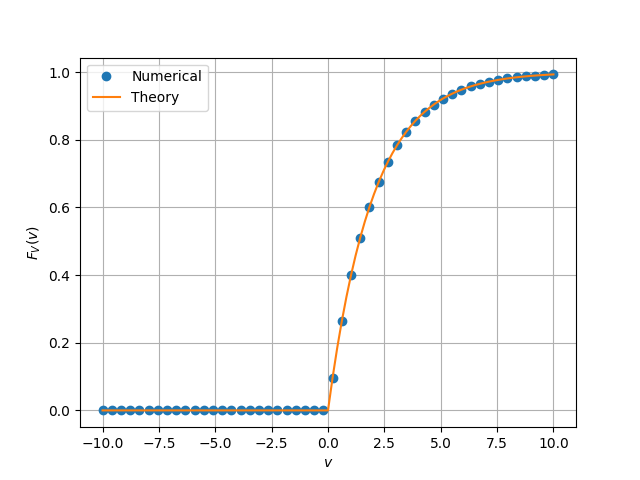
\includegraphics[width=\columnwidth]{V_cdf.png}
    \caption{The CDF of $V$}
    \label{fig:V_cdf}
\end{figure}

\item Find a theoretical expression for $F_V(x)$.

\begin{align}
    F_V(x) &= Pr(V \le x)\\
    &= Pr(-2 ln(1-U) \le x) \\
    &= Pr(U \le 1-e^{-\frac{x^2}{2}}) \\
    Pr(U<x) &= \int_0^x dx = x \\
    \therefore Pr(U \le 1-e^{-\frac{x^2}{2}}) &= 1-e^{-\frac{x^2}{2}} \\
    \rightarrow F_V(x) &=1-e^{-\frac{x^2}{2}}
\end{align}
%

\end{enumerate}

\end{document}